% Problem 2
\subsubsection{2.} 함수 $f\left(x\right)=\dfrac{k}{1+x^2}$이 모든 실수 범위에서 확률밀도함수가 되기 위한 상수 $k$를 구하고, 확률 $P\left(\dfrac{1}{\sqrt{3}} \leq X \leq 1\right)$을 구하라.

\paragraph{Solution.} 모든 실수 범위에서 $f\left(x\right)$가 확률밀도함수가 되려면, $\displaystyle \int_{-\infty}^{\infty} f\left(x\right) \mathop{dx} = 1$이어야 한다.

\begin{align*}
	& \int_{-\infty}^{\infty} f\left(x\right) \mathop{dx}\\
	&= \int_{-\infty}^{\infty} \dfrac{k}{1+x^2} \mathop{dx}\\
	&= k \left[\lim_{t\rightarrow-\infty} \int_{-\infty}^{0} \dfrac{1}{1+x^2} \mathop{dx} + \lim_{t\rightarrow\infty} \int_{0}^{\infty} \dfrac{1}{1+x^2} \mathop{dx}\right]\\
	&= k \left[\lim_{t\rightarrow-\infty} \left.\tan^{-1}x\right|^0_t + \lim_{t\rightarrow\infty} \left.\tan^{-1}x\right|^t_0\right]\\
	&= k\pi
\end{align*}

$k\pi = 1$이므로, $k = \dfrac{1}{\pi}$이다.

또한 이 때 $P\left(\dfrac{1}{\sqrt{3}} \leq X \leq 1\right)$는 

\begin{align*}
	& P\left(\dfrac{1}{\sqrt{3}} \leq X \leq 1\right)\\
	&= \int_{\frac{1}{\sqrt{3}}}^{1} f\left(x\right) \mathop{dx}\\
	&= \dfrac{1}{\pi}\left.\tan^{-1}x\right|^1_{\frac{1}{\sqrt{3}}}\\
	&= \dfrac{1}{\pi}\left(\dfrac{\pi}{4} - \dfrac{\pi}{6}\right) = \dfrac{1}{12}
\end{align*}

이 된다.

% Problem 5
\subsubsection{5.} 다음 확률밀도함수에 대한 분포함수 $F\left(x\right)$를 구하고, 확률 $P\left(3 \leq X \leq 7\right)$을 구하라.
\[f\left(x\right) = \left\{
\begin{array}{ll}
	\dfrac{1}{10} & \qquad 0\leq x\leq 10 \\
	0 & \qquad\textrm{다른 곳에서}
\end{array}
\right. \]

\paragraph{Solution.} 분포함수 $F\left(x\right)$는 밀도함수 $f$를 적분해 얻을 수 있다. 따라서 
\[F\left(x\right) = \left\{
\begin{array}{ll}
	0 & \qquad x\leq 0 \\
	\dfrac{x}{10} & \qquad 0\leq x\leq 10 \\
	1 & \qquad 10\leq x
\end{array}
\right. \]
이다. 또한 $P\left(3\leq X\leq 7\right)$은 $\displaystyle \int_3^7 f\left(x\right) \mathop{dx} = \dfrac{2}{5}$이다.

% Problem 8
\subsubsection{8.} 생명보험에 가입한 어떤 가입자는 의사로부터 평균 100일 정도 살 수 있다는 통보를 받았다. 그리고 이 환자가 사망할 때까지 걸리는 시간 $X$는 다음과 같은 확률밀도함수를 갖는다고 한다.
\[f\left(x\right) = \left\{
\begin{array}{ll}
	\dfrac{1}{100} e^{-\frac{x}{100}} & \qquad x>0 \\
	0 & \qquad\textrm{다른 곳에서}
\end{array}
\right. \]

\begin{itemize}
  \item [(1)] 이 환자가 150일 이내에 사망할 확률을 구하라.
  \item [(2)] 이 환자가 200일 이상 생존할 확률을 구하라.
\end{itemize}

\paragraph{Solution.} 이 함수의 누적분포함수 $F\left(x\right)$는 다음과 같다.

\[F\left(x\right) = \left\{
\begin{array}{ll}
	0 & \qquad x\leq 0 \\
	1-e^{-\frac{x}{100}} & \qquad x > 0
\end{array}
\right. \]

\begin{itemize}
  \item [(1)] 150일 이내에 사망할 확률: $P\left(X < 150\right) = F\left(150\right) = 1-e^{-1.5} \approx 0.7769$
  \item [(2)] 200일 이상 생존할 확률: $P\left(X \geq 200\right) = 1 - P\left(X < 200\right) = 1 - F\left(200\right) = e^{-2} \approx 0.1353$
\end{itemize}

% Problem 12
\subsubsection{12.} 전기회로의 가변저항 $X$는 다음과 같은 확률밀도함수를 갖는다고 한다.

\[f\left(x\right) = \left\{
\begin{array}{ll}
	kx^2\left(1-x^2\right) & \qquad 1\leq x\leq 2 \\
	0 & \qquad\textrm{다른 곳에서}
\end{array}
\right. \]

\begin{itemize}
  \item [(1)] 상수 $k$를 구하라.
  \item [(2)] 분포함수 $F\left(x\right)$를 구하라.
  \item [(3)] 이 전기저항이 $1.05$와 $1.65$ 사이일 확률을 구하라.
\end{itemize}

\paragraph{Solution.}
\begin{itemize}
  \item [(1)] \begin{align*}
 	&\int_{-\infty}^{\infty} f\left(x\right) \mathop{dx}\\
 	=& \int_{1}^{2} kx^2\left(1-x^2\right) \mathop{dx}\\
 	=& k \left[\dfrac{1}{3}x^3 - \dfrac{1}{5} x^5\right]_1^2\\
 	=& -\dfrac{15}{58}k = 1
  \end{align*}
  $-\dfrac{15}{58}k = 1$이므로 $k = -\dfrac{58}{15}$이다.\\
  \item[(2)] (1)의 적분 과정을 이용하면 \[F\left(x\right) = \left\{
\begin{array}{ll}
	0 & \qquad x < 1\\
	\dfrac{3}{58} x^5 - \dfrac{5}{58} x^3 + \dfrac{1}{29} & \qquad 1\leq x\leq 2 \\
	1 & \qquad x > 2
\end{array}
\right. \]
	이다.
  \item[(3)] $P\left(1.05\leq X\leq 1.65\right) = F\left(1.05\right) - F\left(1.65\right) \approx 0.2791$
\end{itemize}

% Problem 14
\subsubsection{14.} 확률변수 $X$의 분포함수가 다음과 같을 때, 다음 확률을 구하라.

\begin{itemize}
  \item [(1)] $P\left(X=0\right)$
  \item [(2)] $P\left(0<X\leq 3\right)$
  \item [(3)] $P\left(0<X<3\right)$
  \item [(4)] $P\left(4<x\leq 5\right)$
  \item [(5)] $P\left(X\geq 1\right)$
\end{itemize}

\begin{center}
	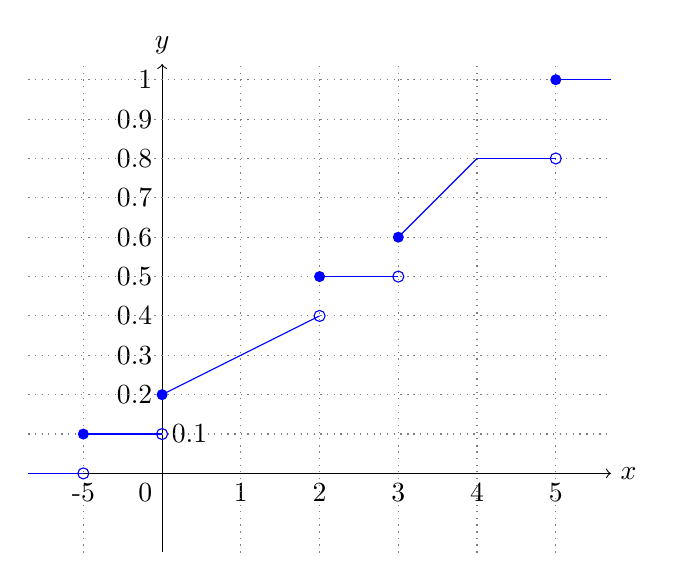
\begin{tikzpicture}	
		\draw[->] (-1.7,0) -- (5.7,0) node[right] {$x$};
		\draw[->] (0,-1) -- (0,5.2) node[above] {$y$};
		
		\node[below left] at (0,0) {0};
		\node[below] at (-1,0) {-5};
		\draw[domain=-1:5.2,smooth,dotted,variable=\y,gray]  plot ({-1},{\y});
		\foreach \x in {1,...,5} {
			\node[below] at (\x,0) {\x};
			\draw[domain=-1:5.2,smooth,dotted,variable=\y,gray]  plot ({\x},{\y});
		}
		\node[right] at (0,0.5) {0.1};
		\draw[domain=-1.7:5.7,smooth,dotted,variable=\z,gray]  plot ({\z},{0.5});
		\foreach \x in {2,...,10} {
			\pgfmathsetmacro\y{\x/10}
			\node[left] at (0,\x/2) {\pgfmathprintnumber[fixed,precision=1]{\y}};
			\draw[domain=-1.7:5.7,smooth,dotted,variable=\z,gray]  plot ({\z},{\x/2});
		}
		
		\draw[domain=-1.7:-1,smooth,variable=\x,blue] plot ({\x},0);
		\draw[domain=-1:0,smooth,variable=\x,blue] plot ({\x},0.5);
		\draw[domain=0:2,smooth,variable=\x,blue] plot ({\x},{\x/2+1});
		\draw[domain=2:3,smooth,variable=\x,blue] plot ({\x},2.5);
		\draw[domain=3:4,smooth,variable=\x,blue] plot ({\x},{\x});
		\draw[domain=4:5,smooth,variable=\x,blue] plot ({\x},4);
		\draw[domain=5:5.7,smooth,variable=\x,blue] plot ({\x},5);
		
		\foreach \Point in {(-1, 0.5), (0, 1), (2, 2.5), (3, 3), (5, 5)}{
    		\fill[fill=blue] \Point circle[radius=2pt];
		}

		\foreach \Point in {(-1, 0), (0, 0.5), (2, 2), (3, 2.5), (5, 4)}{
    		\draw[blue] \Point circle[radius=2pt];
		}
	\end{tikzpicture}
\end{center}

\paragraph{Solution.}
\begin{itemize}
  \item [(1)] $0.1$
  \item [(2)] $0.4$
  \item [(3)] $0.3$
  \item [(4)] $0.2$
  \item [(5)] $0.7$
\end{itemize}

% Problem 15
\subsubsection{15.} 다음 분포함수를 갖는 확률변수 $X$에 대하여 밀도함수 $f\left(x\right)$와 확률 $P\left(X = 1\right)$, $P\left(X<1.5\right)$을 구하라.
\[F\left(x\right) = \left\{
\begin{array}{ll}
	0 & \qquad x < 1 \\
	\dfrac{x^2-2x+2}{2} & \qquad 1\leq x<2 \\
	1 & \qquad x\geq 2
\end{array}
\right. \]

\paragraph{Solution.} $\displaystyle \lim_{t\rightarrow 1^-}F\left(t\right)=0$, $F\left(1\right)=\dfrac{1}{2}$이고, $\displaystyle \lim_{t\rightarrow 2^-}F\left(t\right)=1$, $F\left(2\right)=1$임을 통해 $F$는 $x = 1$에서 불연속임을 알 수 있다. 따라서 $\displaystyle f\left(1\right)=F\left(1\right)-\lim_{t\rightarrow 1^-}F\left(t\right)=\dfrac{1}{2}$이고, 나머지 구간에서는 $F$를 미분해 $f$의 값을 구할 수 있다.

\[f\left(x\right) = \left\{
\begin{array}{ll}
	0 & \qquad x<1 \\
	\dfrac{1}{2} & \qquad x=1\\
	x - 1 & \qquad 1<x< 2\\
	0 & \qquad x\geq 2 \\
\end{array}
\right. \]

그러므로 $P\left(X = 1\right) = f\left(1\right) = 0.5$, $\displaystyle P\left(X<1.5\right) = f\left(1\right) + \int_1^{1.5} f\left(x\right) \mathop{dx} = 0.625$이다.